\documentclass{article}
\usepackage[utf8]{inputenc}
\usepackage{gensymb}
\usepackage{graphicx}
\usepackage{parskip}

\newcommand{\HRule}{\rule{\linewidth}{0.5mm}}

\begin{document}

\pagenumbering{gobble}

\begin{center}

\HRule \\[0.4cm]
{ \huge \bfseries Lab 1: GNSS Single Point Precision Estimation \\[0.4cm] 
\Large \bfseries TTK5: Kalman Filtering and Navigation \\[0.4cm] } 

\HRule \\[1.5cm]

\begin{center} \large
\emph{By:}\\
\textbf{Andreas Nordby Vibeto}\\
andvibeto@gmail.com \\
(andreanv@stud.ntnu.no)
\end{center}

\vfill

{\large \today}

\end{center}
\newpage
\pagenumbering{arabic}

\section*{Task 1}

East North Up (ENU) is a reference frame fixed to the earth surface. Its x-axis points east, y-axis points north and its z-axis points upwards perpendicular to the earth surface. The orign of the frame is on the earth surface relatively close to the object itself. For this reason it is often referred to as a local frame, since it describes the objects position in what can be called a small, limited area. Since the origin is located at the earth surface, the earths curvature must be taken into consideration. This is done by using a reference ellipsoid. The standard ellipsoid for GPS is the WGS-84.

The Earth Centered Earth Fixed (ECEF) reference frame does not have its origin on the earth surface. The origin is in the center of the earth where the x-axis points to the intersection of the 0$\degree$ longitude and latitude, z-axis points to the geographic north along the rotation axis and the y-axis is placed perpendicular to the x- and z-axis. The frame rotates with the earth. When using this frame to describe a postion on the earth surface (or relatively close) longitudenal and latitudinal coordinates are used together with height. For describing objects further away from the surface, like satellites, cartesian coordinates are used.

The two coordinate systems have different usages. Since the ECEF coordinate system rotates with the earth, it is not an inertial coordinate frame. This means that Newton's law of motion cannot be used in this frame. However, it is used to describe the position of objects when the distances are large (i.e. position on earth). For small distances, and when one needs to use Newton's law of motion for an object, ENU is used. Switching between these two coordinate systems is pretty straight forward, which makes it possible to describe an objects motion using the ENU frame, and its position using the ECEF frame. This is very useful when controlling for example a ship or aircraft that moves over large distances.


\section*{Task 2}

Figure \ref{fig:pos_err} shows the position error in the east, north, up (ENU) local frame. It shows that the error in the east and north frame is about the same value. The error in the north position stays close to zero throughout the measurement, while the error in the east position is a bit more off in the beginning but stabilizes towards the end. The position error in the vertical frame up tends to get worse during the timeseries, and for the most part of the measurement is is varying about 10 meters.

\begin{figure}[!ht]
    \centering
    \makebox[\textwidth][c]{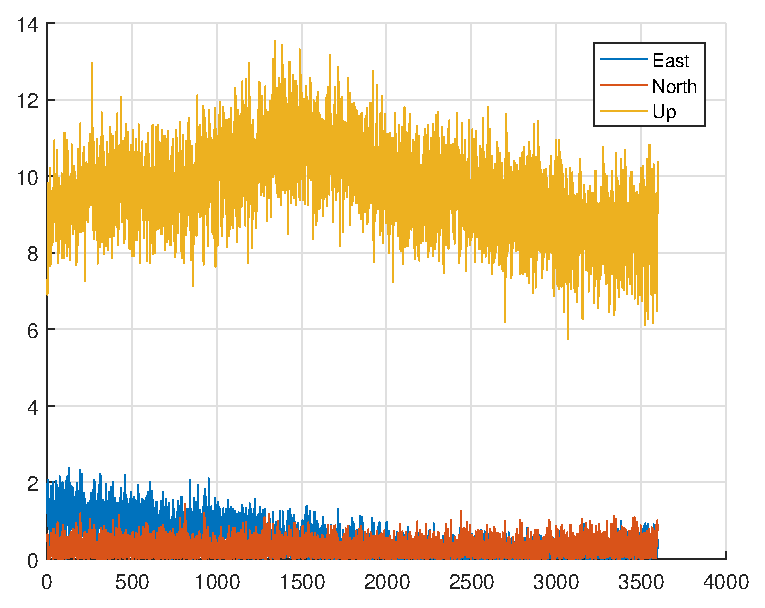
\includegraphics[width=1.25\textwidth, keepaspectratio=true]{../src/error_pos.eps}}
    \caption{Position error in the east, north and vertical frame.}
    \label{fig:pos_err}
\end{figure}

\begin{figure}[!ht]
    \centering
    \makebox[\textwidth][c]{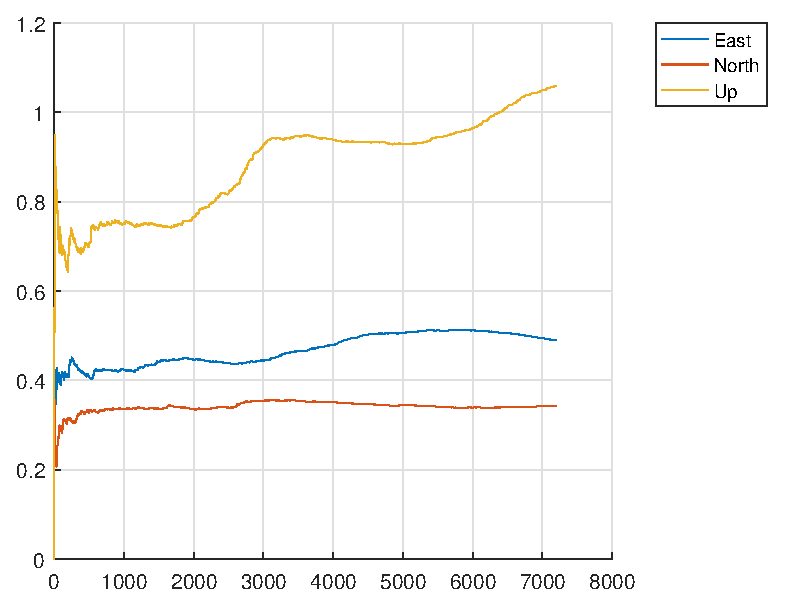
\includegraphics[width=1.25\textwidth, keepaspectratio=true]{../src/std_pos.eps}}
    \caption{Standard deviation of the estimated position in the east, north and vertical frame.}
    \label{fig:pos_std}
\end{figure}

Figure \ref{fig:pos_std} shows the standard devation of the estimated position in the ENU local frame. The standard deviation in east and north direction stays at about $0.4$. In the up direction however, the standard deviation rises pretty much throughout the measurement and is more than one in the end.

The position is calculated using single point position estimation, and weighted least squares to weight the measurements. The algorithm begins every time epoch by determining which satellites is visible. After that the algorithm goes through every step of the calculations ten times, before it updates the position and moves on to the next time epoch. For the weighted least squares calculations elevation dependent variance is used. The standard deviation of the observations has been set to $20$ m, as this is a pretty common deviation for cheaper GPS receivers.

The error in Figure \ref{fig:pos_err} shows the error in meters which is the physical error of the estimated position, the accuracy of the estimation. As the figure shows it varies with a high frequency, about one meter, which comes from inaccuracy in the pseudorange measurements. The standard deviation in Figure \ref{fig:pos_std} relates to the preciseness of the position estimation. The preciseness does not relate to a given error in the position, but relates to how spread out the measurements are. The standard deviation doesn't vary as much as the error. This is because it does not relate to physical variable, instead it describes the dataset as a whole.


\section*{Task 3}
The Dilution of Precision (DOP) is a number that tells you how good estimates of your position the receiver can make. By using the standard deviation of the pseudorange measurements from all the satellites that are being used to calculate position it is possible to get a DOP number that tells how good the receiver can estimate position, and horizontal and vertical position. The DOP can also tell how good the geometrical spreading of the satellites is (satellites further away from each other is better than satellites close to each other). The DOP is a nonnegative number where less than 1 is ideal, but numbers below 5 is acceptable (https://en.wikipedia.org/wiki/Dilution\_of\_precision\_(navigation)).

\begin{figure}[!ht]
    \centering
    \makebox[\textwidth][c]{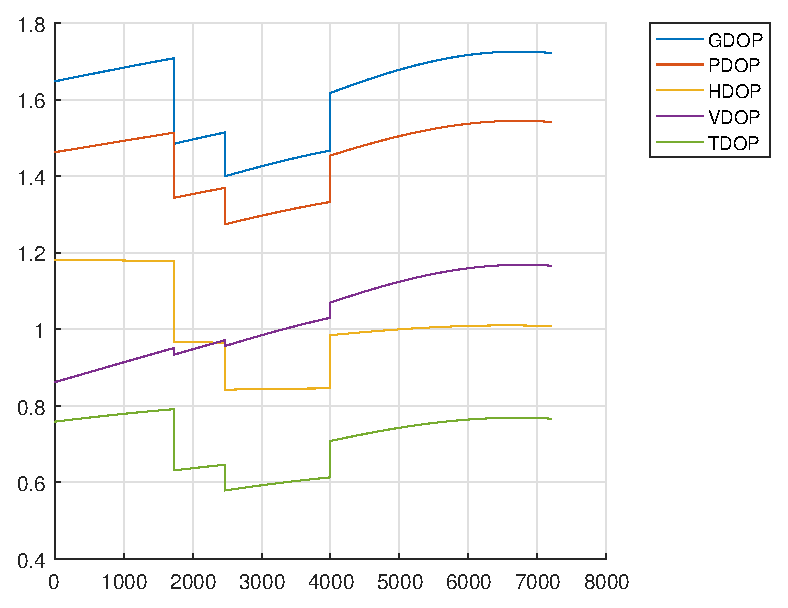
\includegraphics[width=1\textwidth, keepaspectratio=true]{../src/dop.eps}}
    \caption{Dilution of Precision (DOP) values for the GPS measurement}
    \label{fig:dop}
\end{figure}

Figure \ref{fig:dop} shows the different DOP values for the given measurement. In general, the DOP values are very good with none of the exceeding $1.8$. The best is the time DOP never exceeding $0.8$ which means that the receiver can accurately estimate the time error. The horizontal and vertical DOPs are also very good, and they are both better than the position DOP. This is simply because the PDOP is the HDOP and VDOP added together. This also explains why the geometric DOP has the highest value, since it is the result of all the other DOPs added together.

\begin{figure}[!ht]
    \centering
    \makebox[\textwidth][c]{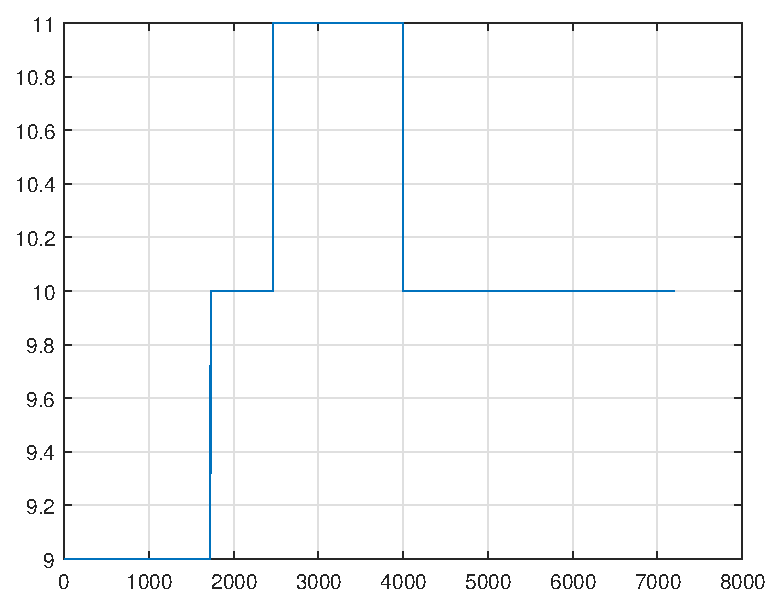
\includegraphics[width=1\textwidth, keepaspectratio=true]{../src/dop_no_satellites.eps}}
    \caption{Number of satellites visible throuhgout the measurement.}
    \label{fig:no_satellites}
\end{figure}

The most interesting result that can be seen from the DOPs is that they all improve a bit at approximately 1800, improve even a bit more at approximately $2400$, before they get worse at $4000$. This can be explained with how many satellites is visible at the given time, which is shown in figure \ref{fig:no_satellites}. From the figure it can be seen that at the same time as the DOP values decrease there is an increase in the number of visible satellites, and opposite when the DOPs increase.

The VDOP distinguishes itself from the rest of the values as it tend to increase over the course of the measurement. This leads to that the VDOP is worse at the end of the measurement than it was at the beginning, even though more satellites are visible. This most likely has to do with the position of the satellites. The receiver is able to more accurately estimate the vertical position when the satellites has a low elevation. Since the VDOP increases during the measurement, it is likely that the visible satellites moves to positions with higher elevation during the measurement.

\section*{Task 4}

\begin{itemize}
	\item Space Based Augmentation System (SBAS)
	\item Ground Based Augmentation System (GBAS)
	\item Precise Point Positioning (PPP)
	\item Real Time Kinematics (RTK)
\end{itemize}











\end{document}